\documentclass{article}

\usepackage{nomencl}
\makenomenclature

\usepackage{amsthm}
\usepackage{amsmath}
\usepackage{graphicx}
\usepackage{subfigure}
\usepackage{verbatim}
\usepackage[toc]{glossaries}
\usepackage{epstopdf}

\usepackage{algorithm} 
\usepackage{algorithmic}

\newtheorem{theorem}{Theorem}[section]
\newtheorem{corollary}[theorem]{Corollary}
\newtheorem{defination}{Definition}[section]
\newtheorem{proposition}{Proposition}[section]

\begin{document}
\nomenclature{MAC}{Message Authentication Code: A short message block generated
with message protected. MAC is concatenated to the rightmost of the message in
transmission}
\nomenclature{Tag}{The output short block of a MAC generation scheme}
\nomenclature{(M,T)}{Message M and its tag T}
\nomenclature{TG(M, $\ldots$)}{A MAC Scheme processing the message M with
secret information in the arguments list}
\nomenclature{VF(M,T, $\ldots$)}{Verify the message M and tag T with the secret
information in the arguments list. Return 1
if TG(M,$\ldots$) = T and 0 if not.}
\nomenclature{UF-CMA}{Unforgeability under adaptive Chosen Message Attack}
\nomenclature{Pr[A]}{The probability that event A happens}
\nomenclature{Forgery(MAC, A)}{Forgery experiment on a MAC scheme with the
adversary A. Return 1 if A succeed a forgery attack otherwise 0}
\nomenclature{Forgery$_{MAC}$}{The probability that Forgery(MAC, A)=1 for an
adversary A and a MAC scheme}
\nomenclature{PRF}{Pseudo-random Function}
\nomenclature{PRP}{Pseudo-random Permutation}
\nomenclature{Adv$^{F0}_{F1}$}{The probability for an adversary to
distinguish between two functions F0 and F1}
\nomenclature{$\oplus$}{Bitwise exclusive-xor operation(XOR)}
\nomenclature{F$_k$(M)}{Function F processing input M with secret information k}
\nomenclature{E$_k$(M)}{Encrypt input M with secret key k}
\nomenclature{Block Length}{The number of bits of a block}
\nomenclature{Len(M)}{The block length of block M}
\nomenclature{GF-mult(A,B)}{Galois Field multiplication with A and B}
\nomenclature{Tom}{A concatenated to the leftmost of B}
\nomenclature{Tom}{A concatenated to the leftmost of B}
\nomenclature{Tom}{A concatenated to the leftmost of B}
\nomenclature{Tom}{A concatenated to the leftmost of B}
\nomenclature{Tom}{A concatenated to the leftmost of B}
\nomenclature{Tom}{A concatenated to the leftmost of B}
\nomenclature{Tom}{A concatenated to the leftmost of B}
\nomenclature{Tom}{A concatenated to the leftmost of B}
\nomenclature{Tom}{A concatenated to the leftmost of B}

\printnomenclature
\section{Notations and Definitions}
In this part we firstly depict the notations of symbols used to describe Cost-Effective Tag Design(CETD) and the MAC scheme adopted, CETD-MAC. Then we present the security definition of MAC schemes in computational scenario.
%define terms
\subsection{Notations of Symbols}
Let \{0,1\}$^n$ be the set of all n-bit binary strings.  The set of all binary string is expressed as \{0,1\}$^*$.  
For a string M $\in$ \{0,1\}$^n$, Len(M) is its length in bits, and Len(M)$_l$ = $\lceil$Len(M)/l$\rceil$ is the number of l-bits blocks M consist of.  Let 0$^l$ and 1$^l$ denote l-bits strings of all zeros and all ones. 
For a bit string M and an integer l that Len(M) $\geq$ l, msb$_l$(M) denotes the most significant l bits(left most l bits) of M and lsb$_l$(M) for least significant l bits(right most l bits) of M.
For two bit string X and Y, we denote X$\|$Y  or XY as the their concatenation. For bit string M whose length in bits is multiple of integer l, we denote X parted into l-bit sub-strings as X = (X[1]X[2]$\ldots$X[n])$_l$, where X[1], X[2], $\ldots$, X[n] $\in$ \{0,1\}$^l$.

The block cipher encryption of a string X with a secret key K is denoted as E$_K$(X). E$_K$(X) expresses the String mapping of \{0,1\}$^n$ $\rightarrow$ \{0,1\}$^n$ where n is the Len(X) and Len(output).

\subsection{Security Definition of Memory Integrity Protection Designs}
%The practical behaviour of adversary in attacking the integrity
\paragraph{Threat Model} %how the adversary attack the integrity
The attacks discussed in this article mainly situated on the probing and
tampering the data transferred between chip and external memory. In this scenario, the adversary can conduct types of attacks on the (ciphertext, tag) pair stored on the external memory or in the transformation between chip and memory. We call these two types of integrity attack content modification attack and copy-then-replay attack. 

When conducting a content modification attack, then adversary modifies the content of a (ciphertext, tag) pair, (C$_{origin}$, T$_{origin}$). At least one of ciphertext and tag in the modified memory frame (C$_{fake}$, T$_{fake}$) are distinct to the original one sent from the chip. When the chip reads the modified pair (C$_{fake}$, T$_{fake}$), this pair is verified by VF(C$_{fake}$, T$_{fake}$, $\ldots$). If VF(C$_{fake}$, T$_{fake}$, $\ldots$)=1, then the modified pair passes and the content modifying attack succeeds. 

For a copy-then-replay attack, we make the following denotions first:
\begin{itemize}
	\item A$_{origin}$: The address of the external memory frame M attacked 
	\item A$_{copy}$: The address of the external memory frame M1 which is copied by the adversary as the fake frame
	\item TS$_{origin}$: The generation time stamp of the external memory frame M attacked
	\item TS$_{copy}$: The generation time stamp of the external memory frame M2. M2 and M has same address while TS$_{M2}$ is previous of TS$_M$ 
\end{itemize}
During a copy-then-replay attack on a memory frame M whose address is A$_{origin}$ and time stamp is TS$_{origin}$, the adversary A replace M with a copy. This copy can be a frame from other address A$_{copy}$ or one at same address but copied at an old time stamp TS$_{copy}$. The copy is a valid pair from the chip. 
When the chip reads the modified frame (C$_{fake}$, T$_{fake}$), the fake pair(C$_{fake}$, T$_{fake}$) is verified by VF(C$_{fake}$, T$_{fake}$, $\ldots$) and the copying-then-replying attack succeeds if VF(C$_{fake}$, T$_{fake}$, $\ldots$)=1.  

If the fake pair from the adversary passes the verification, the integrity of the data is broken. To defend content modification attack, the MAC scheme should ensure that when the secret information used in tag generation collides for two distinct input data, the related two tags should have low probability to be identical. For copying-then-replaying attack, identical input data should have low probability to lead to tag collision if the secret information used in tag generation are distinct. 

\paragraph{The Security Analysis of Memory Integrity Protection Design}

%the security definition and evaluation standard in computational model
\subsection{Security Definition of MAC Schemes}
In this part we depict the security definition of MAC schemes in computational model.  
%the adversary can choose message other than just brute-force
\paragraph{MAC and proposition 2.7}
\paragraph{Chosen Message Attack}
%in chosen-message attack, the adversary know the relationship and can choose input to enhance passing rate 
The brute-force attack on the integrity of memory frame can be expressed as the following steps:
\begin{itemize}
	\item Randomly pick a memory frame
	\item Keep the ciphertext(or the tag) fixed, then tranverse all the possible tag(or ciphertext) until
\end{itemize}

Goldwasser et al. introduced the concept of unforgeability of chosen message attack in \cite{}. The adversary can select numbers of valid ciphertext-tag pairs, observe the relationship between each ciphertext and its tag, then send a fake ciphertext-tag pair to the verification stags based on the observation.The adversary A1 conducting chosen-message attack is more strategical compare with the one A2 for brute-fore attack in content modification scenario, which means A1 can try less number of ciphertext-tag pairs to pass the verification. 
For instance, if there is a type of relationship between ciphertext and tag for a MAC scheme, A1 will realise this relationship and conduct two types of attack with high probability of passing: just modifying ciphertext from C1 to C2 and C2 has high probability to generate same tag T1; or send new pair (C2,T2) to the verification where C2 and T2 meet the relationship. In A1`s eyes, for given ciphetext C and a unknown nonce N, the tags in the tag domain has different probability to pass the verification while the probability is identical to A2. 

In this article, we assume the adversary can choose the ciphertext in both content modification and copy-then-replay attack. The adversary aims to find groups of inputs that the two inputs from same group has probability of tag collision that is much larger than 1/2$^n$, where n is Len(tag). 

%the theoretical behaviour of the adversary under each attack
\paragraph{Security Analysis Model}%how to conduct attack and analysis the security
In our security analysis of CETD-MAC scheme, the adversary A has access to the tag generation scheme and verification scheme. A can send chosen ciphertexts to the tag generation scheme and determine whether the nonce for his chosen ciphertexts are fixed or not. He can acquire the value of the tag for each his chosen ciphertext while cannot access the value of the related nonce. After analyzing several valid ciphertext-tag pairs, A sends his fake pair (C$_{fake}$, T$_{fake}$) to the verification scheme. The verification scheme generates the tag T of C$_{fake}$ and the fake pair passes the verification if T is identical to T$_{fake}$. Our security analysis on CETD-MAC is modeled like this:
\begin{itemize}
	\item For content-modification attack, the adversary A fixes the nonce and inputs distinct ciphertexts to the tag generation scheme. 	
	\item For copying-then-replaying attack, the value of ciphertexts are fixed to a value C chosen by A. A inputs C continually and as the tag generation scheme to maintain the nonce distinct for each input.    
\end{itemize}
After several rounds of inputing, the adversary analyses the value of tags for his chosen inputs then sends his fake pair(C$_{fake}$, T$_{fake}$) to the verification scheme.   	

%how the adversary choose message in spoofing scenario
\paragraph{Content Modification Scenario}
In content modification scenario, the nonce value is fixed and kept in the trusted area and is unaccessible to the adversary. The adversary tries to replace the valid memory frame (C$_{origin}$, T$_{origin}$) with his fake pair (C$_{fake}$, T$_{fake}$). The forgery advantage F$_{CETD-MAC}$ under content modification attack is the probability that the adversary can get the verification oracle to accept his fake cipehrtext-tag pair. 
%copy-then-reply
\paragraph{Copy-then-Replay Scenario}
In copy-then-replay scenario, the encryption key is maintained unchanged while the nonce value is updated for each calling of tag generation oracle. Secret key and nonces are kept in trusted area and cannot be acquired by the adversary. The adversary can copy the message-tag pairs in old time stamp. When conducting the replay attack, the adversary replaces a memory frame containing a data-tag pair in new timestamp with a copy from his storage. The forgery advantage F$_{CETD-MAC}$ under replay attack is the probability that the adversary can get the verification oracle to accept the replace data-tag pair.  

Assume the copy with old timestamp from the adversary is expressed as (M,T1) where M is the message and T1 is the corresponding tag, and the nonce of (M,T1) is denoted as N1. When applying M to the tag generation at a new time point, we mark the corresponding tag T2 and the nonce N2. If the adversary can succeed a replay attack, then T1 is identical to T2 regardless of the equality of N1 and N2.
Then F$_{CETD-MAC}$ under replay attack can be denoted as the probability Pr[T1 = T2 $\mid$ Message value is M \& N1,N2 are randomly generated]. 

%According to the design of CETD-MAC, the tag can be expressed as Y[1]$\oplus$Y[2]$\oplus$$\ldots$$\oplus$Y[x], x is the number of input sub-blocks to CETD-MAC. If the following equation is met:
%Y$_1$[1]$\oplus$Y$_1$[2]$\ldots$$\oplus$Y$_1$[x]$\oplus$Y$_2$[1]$\oplus$Y$_2$[2]$\ldots$$\oplus$Y$_2$[x] = 0, where Y$_1$ blocks produce T1 and Y$_2$ blocks generate T2, then T1 is identical to T2. This equation indicates that the behaviour of block-level rotate shifting stage effect the probability of tag collision directly. For easy understanding, we firstly analyze the case that shuffle stage does not work under replay attack, which means X$_1$[i] is identical to X$_2$[i] for any i$\in$[1,x]. The analysis of effect from shuffle stage on X blocks follows then.
%
%In replay attack, the adversary replace the memory frame written in new time
%point Time$_2$ with a copy from old time stamp Time$_1$. The content in memory
%frame is a data-tag pair. To defend the replay attack, a tuple(address, counter,
%random number) is adopted as input to block cipher encryption to generate the
%nonce, which serves the control parameter for each stage in tag generation. The
%tuple is distinct for each data message. Assume the block cipher adopted behaves
%like PRF, the nonce under replay attack is random and distributed
%uniformly for each data message. To Cost-Effective Tag design, the security of integrity of data message replys on the
%security of CETD-MAC scheme.


%what is CETD-MAC? what security conclusion has been made?

%\documentclass{article}
%\usepackage{amsthm}
%\usepackage{amsmath}
%\usepackage{graphicx}
%\usepackage{subfigure}
%\usepackage{verbatim}
%\usepackage{glossaries}
%\usepackage{algorithm} 
%\usepackage{algorithmic}
%\usepackage{epstopdf}
%\newtheorem{theorem}{Theorem}[section]
%\newtheorem{corollary}[theorem]{Corollary}
%\newtheorem{defination}{Definition}[section]
%\newtheorem{proposition}{Proposition}[section]

%\DeclareMathOperator*{argmin}{argmin} //argmin或argmax公式的排版
%\enewcommand{algorithmicrequire}{extbf{Input:}} //Use Input in the format of Algorithm
%\enewcommand{algorithmicensure}{extbf{Output:}} //UseOutput in the format of Algorithm
%\begin{document}
%breaking the security result in orignal design and prove that it is not secure under both attacks
\section{Security Analysis of CETD-MAC}
In this section we analysis the security of cost-effective tag design. We firstly introduce our security evaluation model of tag design. This model splits the security analysis into two steps: scheme security and implementation security. We analysis 
%cetd-mac is not secure

\subsection{Computational Based Security Analysis of CETD-MAC}
In this section we discuss the security of CETD-MAC under two tpyes of integrity attack.  The adversary is assumed to know the length of ciphertext and tag on the memory frame he acquired. 
We prove that the probability that the fake pair passes the verification scheme under both two attacks is determined by the proportion of the 1s and 0s in the input ciphertexts and provide the equations quantifying this relationship. This fact indicates that the adversary can choose special ciphertext-tag pairs which have higher probability to pass the verification compared with other pairs.  

%in this case nonce is fixed and serves as the key as the deterministic MAC schemes
%the number of queries to succeed a forgery attack can be at most 2^{n-1}
In the computational model based security analysis on MAC schemes, a secure MAC scheme should ensure that for any two input messages in the domain, the probability that their tags collide should be no more than an upper bound. This definition of secure MAC scheme is widely accepted and has been adopted in the security analysis of iterated MAC schemes such as CBC-MAC \cite{} and its variants \cite{}, and parallel MAC schemes such as PMAC \cite{} and its variants\cite{}. This definition emphasizes that when the key used in the MAC scheme is unaccessible to the adversary, the adversary cannot find any relationship between a given tag and a given input message. In the eyes of the adversary, a given tag can be generated by any message in the input domain and for a given input message, its tag can be any one value in the tag range. 
\subsubsection{Content Modification Attack Scenario}
In this part we prove that for CETD-MAC, the input ciphertexts have relationship between their tags.  For a given tag, the number of possible inputs is limited and can be computed based on the tag value. On the other hand, for a give input ciphertext, the number of possible tag value is also limited and can be computed based on the ciphertext value. This fact indicates that when modifying the ciphertext part C1 of a memory frame, the number of possible ciphertexts C2 to replace C1 is limted. On the other hand, the adversary can manifast the fake ciphertext-tag pair C$_{fake}$-T$_{fake}$ based on the relanship between a ciphertext and its tag quantified in thei part and win a much high probability to pass the verification stage compared with randomly choosing a ciphertext and a tag. 

When conducting content modification attack, the adversary modifies the content of a memory frame from (C, T) to (C1, T1). When the verification stage VF read the modified (C1, T1) pair, VF computes C1`s tag, marked as T$_{tmp}$, using the nonce N which is also used in computing T. If T$_{tmp}$ is identical to T1, then the content modification attack succeed. We can see that in content modification attack, for two pairs (C$_{origin}$, T$_{origin}$) and (C2, T1), their nonce N and N1 are identical. To succeed the content modification attack, the adversary will choose the C1 that has high probability to get tag value T    
\paragraph{The Diffusion Does Not Introduce New Bits}
In CETD-MAC scheme, the shuffle and shift stage relocate bits in the ciphertext to new index. Even though the new index of each bit in the cihpertext is unpredictble as the nonce is the output of a PRF and unaccessable to the adversary, it is certain the output of shift shuffle and shift stage contain same bits as the ciphertext. Assume ciphertext is consist of m blocks each of whose length is n bits, and there are totally k 1s in the m*n bits in the ciphertext. The the output of shuffle and shift stage also have k 1s and m*n - k 0s. 

As mentioned before, the 0-1 proportion is maintained during the shuffle and shift operation. That means if two distinct ciphertext C1 and C2 have same proportion, marked as k/m*n-k, the 0-1 proportion in their corresponding shift outputs Y1 and Y2 is also k/m*n-k.  
If we fix a nonce and keep querying ciphertext with same 0-1 proportion, the outputs of shift stage can be regarded as a seg of m*n bits messages with same 0-1 proportion but uncertain bit distribution. If a ciphertext has k 1s, then the distinct ciphertexts have k 1s form a set S$_{n}^{k}$ and the set size is $\binom{n}{k}$, marked as C$_{n}^{k}$. The ith element in set S$_{n}^{k}$ is marked as C[i] and the tag of C[i] is T[i].   
We fix a nonce N for the set S$_{n}^{k}$ and compute T[1]. We discuss possbile distribution of k 1s in m Y blocks according to the value of k compared with m*n to see the number of possible distinct values of T1. 

Firstly, we assume k is no larger than n. When xoring Y blocks to generate T[1], the jth bit of T[1], marked as T[1][j], is computed as T[1][j] = Y1[1][j]$\oplus$Y1[2][j]$\oplus$Y1[m][j], where Y1[i][j] is the jth bit in the ith Y block. We call the jth bit in all Y blocks a jth colunm. The jth bit of T1 is formed by xoring all the bits in the jth column of Y block.  It is obvious that T1 can have at most k 1s and the number of distinct T1 with k 1s is $\binom{n}{k}$. In this case all the k 1s distribute in distinct k columne.  If we want new value of T1, we need to move one of 1 to another column. This relocation reduce the number of 1s in T1 from k to k-2, leading to $\binom{n}{k-2}$ new distinct values of T1. If we want more new values, we need to keep move 1s to another column like this way and each time of relocation reduce 2 1s in T1, which means the possible number of 1s in T1 canbe k, k-2, k-4,$\ldots$, 0(if k is even) or 1(if k is odd). Then we draw the following Theorem:
\begin{theorem}
Assume a ciphertext consist of m n-bits blocks has k 1s and k is no larger than n, then the the number of possible distinct value of its tag when the nonce is unaccessible is compute with the equation:
No of distinct tags is $\sum_{i=0}^{k/2}$ $\binom{n}{k-2*i}$ if k is even or $\sum_{i=0}^{(k-1)/2}$ $\binom{n}{k-2*i}$ if k is odd
\end{theorem}
When k is identical to n or n-1, the number of distinct tags is 2$^{n-1}$.  

If k is larger than n and no larger than m*(n-1), for any k in this domain, it is possible to generate a tag containing 0 to n 1s. That means for any k $\in$ [n, m*(n-1)], the number of possible distinct tags for a ciphertext is 2$^{n-1}$. 

When k is larger than m*(n-1), the way to compute number of possible distinct tags is simular to the case that k is no larger than n. In this case, the tag can has at most n - (k mod n) 0s the value with less number of 0s can be acquired by overlapping 0s in one column. The number of possible distinct tag values can be computed with the following equation:
No of distinct tags is $\sum_{i=0}^{(m*n-k)/2}$ $\binom{n}{()k-2*i}$ if k is even or $\sum_{i=0}^{(m*n-k+1)/2}$ $\binom{n}{k-2*i}$ if k is odd

%give Theorem of content modificatoin attack
\paragraph{The Relationship Between Ciphertext and Its Tag}
If the MAC scheme is ideal and behaves like a PRF, for any input ciphertext, the probability that its tag equals to a specific value is 1/2$^n$, where n is Len(tag). 
As the both shuffle and shift subroutines in CETD-MAC scheme are diffusion operations, for each input ciphertext, its 0-1 proportion will be maintained until the xor subroutine. This fact means that for a specific input ciphertext, the number of its possible tag values is limited. For example, assume the input ciphertext is 0x 
\paragraph{Input can be divided into groups}
%Given a ciphertext and unknown nonce, the number of tags that a adversary needs to try is determined by the number of 1s in the ciphertext, this property can help the adversry contrive strategry to reduce the number of guessing.
%on the other hand, the adversary can deisgn its c-t pair according to this property. 
%besides same proportion ciphertext, what type of other ciphertext can the advesrary to use with high prob of passing?
\paragraph{Forgery Attack on CETD-MAC in Content Modification Scenario}
In content modification attack, the adversary acquires a valid memory frame and try to modify the content. If the adversry knows the length of ciphertext and the tag, he will know the value of the ciphertext and the tag. According to the previous analysis on the relationship between bit proportion and possible tag values, the adversary can conduct the following two types of modification on the frame:
\begin{enumerate}
	\item Select a new ciphertext that has T$_{origin}$ in its possible tag domain. A better choice is to select a ciphertext with same number of 1s as the tag T$_{origin}$
	\item Replace the frame with a new pair (C2, T2) that T2 is in the possible tag domain of C2
\end{enumerate}
From Theorem $\ref{}$ we know that if the number of 1s in m*n bits is to large(more than m*(n-1)) or too small(less than n), the possible tag domain size is small. This fact 

%input is fixed and the nonce changes for each query,
%the number of query
\subsubsection{Copy-then-Replay Attack Scenario}
When conducting copy-then-replay, the adversary replace a valid memory frame with his stored copy of a frame from other address or same address but older time point. The probability that the adversary succeed the copy-then-replay attack is determined by the probability that for a fixed input C, the two tags T1 and T2 are identical when their nonce N1 and N2 are randomly generated.

As depicted in Section $\ref{}$, the 0-1 proportion of a ciphertext is maintained to the output blocks(Y blocks) of shift stage. This fact means for a fixed input, the Y block set Y1 and Y2 for two randomly generated nonce N1 and N2 have same 0-1 proportion.  
\paragraph{Copy-then-replay}
\paragraph{Forgery Attack on CETD-MAC in Copy-then-Replay Scenario}
As the probability that two tags collide when their inputs are identical and their nonce are randomly generated is determined by the 0-1 proportion of their inputs, the adversary can just attack the frame with the copy whose ciphertext has many 1s(more than m*(n-1)) or few 1s(fewer than n). Two extrame case is all 0 and all 1 ciphertexts, no matter what nonce is adopted, their tags will always be 0.

%it is impossible to modify cetd-mac with existing operations to enhance security
\subsection{Security Enhancement of CETD-MAC with Its Operations}
In this part we try to enhance the security of CETD-MAC without introducing new operations or data. We analyze the functionality of each operation first and discuss whether it is necessary to maintain each operation in the new design.
%why to add each operation, why unsufficient to use each only ?
\subsubsection{Design Rationale of Original CETD-MAC Scheme}
CETD-MAC scheme is consist of three stages: bit-segment shuffle with user chosen shuffle round, then cycle shift for each output lf shuffle stage with randomly chosen shift length and finally xor all output block of shift stage to the tag. It is insecure to construct with only one of the three stages.
\paragraph{XOR stage}
The xor operation is a common choice for parallel MAC schemes to convert m n-bits block to a n-bits tag. It has been analyzed by Bellare in \cite{} that it is insecure to construct a MAC scheme with xor operation only as simply swapping the order of two blocks in the input can lead to tag collision.  The input blocks must be processed before sent to xor stage to ensure that simply changing the order of two input blocks in the input will change the input set of xor stage.
\paragraph{Cycle Shift Stage}
In original CETD-MAC scheme, cycle shift stage, short for shift stage, locates before the xor stage. For each input block of shift stage, the number of bits shifted is determined by the value of a nonce segment. Shift stage can defend the attacks such as changing the order of two input blocks as the adversary has no access to the nonce value and then can not predict the number of bits shifted of each block, then has no idea that changing the order of which two blocks lead to tag collision with high probability. However, it is still insecure to construct a MAC scheme by adopting shit stage then xor stage, as for some input blocks which are consist of one kind of patterns, shifting different number of bits can still lead to same output block. This fact means that reordering the blocks formed by a pattern have higher probability to lead to tag collision than other blocks. This fact is depicted in detail in Appendix $\ref{}$. 

%why it is unsufficient to use shuffle only if the number of blks are large?
\paragraph{Bit-Segment Shuffle Stage}
Shuffle stage swaps two bit-segments in each round. As the index and offset of swapping in each round is determined by the nonce, the adversary cannot predict which blocks participate the shuffle. One problem to use shuffle without shift is that if the number of blocks are large while the number of shuffle round is small, the number of blocks participating the shuffle is small. This fact is serious in copy-then-replay attack as majority of blocks may not participate shuffle and the content of these unshuffled blocks will be maintained until the next stage. If the operation linked to shuffle is the xor stage directly without shift stage, according to Equation $\ref{}$ we can see that the probability of tag collision is determined by th

and the adversary can repeat some blocks in the input as he wish to enhance the collision probability of the output from shuffle.  In the original CETD-MAC, the shift stage will help re-ordering the bits in the output blocks from shuffle stage to ensure that the input blocks of xor stage is hard for the adversary to predict. 

\paragraph{Diffusion is insufficient to construct a secure MAC scheme}
%linearity analysis and different analysis
We can see what shuffle and shift do is reordering the bits in the input message
blocks. We give each input bit a index from 1 to m*n. When the nonce is fixed
and unknown, we are certain for two inputs M1 and M2 the bits with same index
will be relocated to same new index. The adversary does not know the exact bit
distribution of the input blocks to xor stage but he knows that the 0-1
proportion is same as the input of CETD-MAC. As depicted in Section $\ref{}$, the odd-even property of the tag is identical to its input, and the number of possible distinct tag values can be predict based on the number of 1s in the input. When realized this fact, the adversary just needs to choose a tag value that has same odd-even property and the number of 1s is no more than min(n,k), there k is the number of 1s in the input.

Content Modification Scenario
In content modification scenario, the adversary keeps modifying a memory frame in an address until the frame passes verification. The modification will be previous to the next write operation from the chip the same address. 

Copy-then-Replay Scenario
To eliminate this weakness, we need to add a operation to make sure that if the adversary does not know the value of the fixed nonce, he cannot predict the 0-1 proportion and bit distribution of the input blocks of xor stage. 
%
\paragraph{No-linearity and Random Bit Injection}
In cite{},R and J depicted the design rationale of each operation in Rij AES. Their should be three types of operations in a block cipher design serving as no-linearity, random-bit injection and diffusion.  
In original CETD-MAC scheme, both shuffle and shift operation achieve the diffusion, while no operation can inject random bits for each input and all the operation in the CETD-MAC is linear.  
%block cipher consist of three operations
%no-linearity must be achieved with gf-mult

%new MAC design based on CETD-MAC
\section{Security Improved CETD-MAC}
We have shown that the original CETD-MAC cannot effectively defend two types of integrity attacks as the number of distinct tags is determined by the proportion of 1s and 0s. In this section, we propose several approaches to improve the security of CETD-MAC. Firstly we tried to utilize the nonce and the operation existing in the original CETD-MAC design and then prove the reason that this attempt cannot succeed. Then we proposed our rationale on improvement based on the instruction from \cite{}.  
%we need to add gf-mult to provide no-linearity, gf-mult a nonce seg can do
%random inject together
\paragraph{No-linearity and Random Bits Injection: Approaches in other schemes}
\paragraph{Galois Field Multiplication}
As mentioned in Section $\ref{}$, it is insufficient to use linear operation
only to construct a secure MAC scheme. The reason is that linear operations can
diffuse the bit distribution of the input while can not introduce new bits. On
the ther hand, the input and the output of linear operation has linear
relationship and the adversary can find the relationship and conduct successfule
forgery attack since then without acquiring the nonce or the key.

The we need to add no-linearity random bit injection operation. For the MAC
schemes constructed with block cipher, such as CBC-MAC(and its variants) and
PMAC(and its variants), the block cipher usually contains these two operations.
R and J mentioned in \cite{} the galois field multiplication and its inverse
operation can serve as no-linearity operation. 
For example in Rij AES, the ByteSub provide no-linearity to the input by
adopting the galois multiplication inverse to each input byte then affline
transformation with a constant matrix to the input. Random bits that stored in a
roundkey, which is acquired by expanding the encryption key, is injected to the
input by xoring the roundkey with processed input.  

In GMAC, the author utilized the galios field multiplication other than block
cipher to process each input block serially. Each input block does galois field
multiplication with H, which is acquired by encrypting constant 0 with a secret
key. The output of multiplication is xored with the next input block to serve as
the multiplicand for H. The advantage of multipling each xored input block with
H compared with calling the encryption function to the input block directly is
that the no-linearity and random bit injection is combined to one round
operation, which reduces the space cost and enhances the processing speed.

The application of GF multiplication in GMAC inspired us on the security
optimization of original CETD-MAC scheme as for each ciphertext to be processed,
a nonce is generated with block cipher. The nonce or its segment can serve as
the H in the GF multiplication in GMAC. 
\subsection{Improved CETD-MAC with higher security level}
In this part we introduce our improved version of CETD-MAC. In our first attempt
of improvement, we do galois field multiplication, short for gf-mult, to each input block with a
segment extracted from nonce. We call this first attempt Fully-GFM CETD-MAC as
each input block will participate the galois mulatiplication. We also introduce
its variant named Selected-GFM CETD-MAC in which the number of input blocks
doing gf-mult is determined by user choice, just as what shuffle stage does. 

Adding gf-mult before shuffle can inject random bits to the inputs and the
adversary cannot predict the tag based on the input value according to the
attack strategry depicted in Section $\ref{}$. This improvement works for all
the input value except for all 0 input as the output of 0 gf-mult with any value
will be 0. To address this problem, we introduce our second version of improved
CETD-MAC scheme named Flip-then-GFM CETD-MAC scheme. We randomly flip each input
block and then do selecte gf-mult as we did in the variant of first version. We
will show that our second version of improved CETD-MAC is secure under two types
of integrity attacks in this part. 
\subsubsection{Fully-GFM CETD-MAC}
Our first design draft based on the original CETD-MAC are described in
Algorithme $\ref{}$. We name this design Fully GF-Mult CETD-MAC, which mean each
input will do galois field multiplication with a nonce segment.  
\paragraph{}
\paragraph{Selected-GFM CETD-MAC}

\subsubsection{Flip-then-GFM CETD-MAC}

\paragraph{Block Flipping}
\subsection{Our Optimization of Original CETD-MAC}
\paragraph{Defending Content Modification Attack}
Hence the adversary can know the possible input set for a given tag , he can modify the content of ciphertext on the frame to a fake one that has same number of 1s as the tag and this way of modification has highest passing probability. On the other hand, as he knows the possible tag set for a given ciphertext, he can choose the tag for his fake ciphertext`s set to evade the tag values that can not be generated with C$_{fake}$ with any nonce. 

To eliminate these advantage that left to the adversary by the original CETD-MAC, one idea is to make the relationship of 0-1 proportin between cipehrtext and its tag unpredictable if the nonce is unknown. 

%to defend 1st type content modification, we need to ensure that if the nonce is rnd and unkonwn, the size of tag domain is 2^n and if the nonce is rnd, pr[T = k] = 1/2^n for any k 
%to defend 2nd type content modification, we need to ensure that if the it is same as 1st
As the 0-1 proportion of the tag is determined by its input ciphertext, we need to ensure that no matter how we modify the input, the value of the tag for the modified input is unpredictable. Th 

\renewcommand{\algorithmicrequire}{ \textbf{Input:}} %Use Input in the format of Algorithm
\renewcommand{\algorithmicensure}{ \textbf{Output:}} %UseOutput in the format of Algorithm
\begin{algorithm}[htb] 
\caption{Fully Galois Field Multiplication} 
\label{alg:fully-GFM} 
\begin{algorithmic}[1] %这个1 表示每一行都显示数字
\REQUIRE ~~\\ %算法的输入参数:Input
The set of positive samples for current batch, $P_n$;\\
The set of unlabelled samples for current batch, $U_n$;\\
Ensemble of classifiers on former batches, $E_{n-1}$;
\ENSURE ~~\\ %算法的输出:Output
Ensemble of classifiers on the current batch, $E_n$;
\STATE Extracting the set of reliable negative and/or positive samples $T_n$ from $U_n$ with help of $P_n$; 
\label{ code:fram:extract }%对此行的标记,方便在文中引用算法的某个步骤
\STATE Training ensemble of classifiers $E$ on $T_n \cup P_n$, with help of data in former batches; 
\label{code:fram:trainbase}
\STATE $E_n=E_{n-1}\cup E$; 
\label{code:fram:add}
\STATE Classifying samples in $U_n-T_n$ by $E_n$; 
\label{code:fram:classify}
\STATE Deleting some weak classifiers in $E_n$ so as to keep the capacity of $E_n$; 
\label{code:fram:select}
\RETURN $E_n$; %算法的返回值
\FOR{each $i \in [1,9]$}
\STATE initialize a tree $T_{i}$ with only a leaf (the root);\
\STATE $T=T \cup T_{i};$\
\ENDFOR
\FORALL {$c$ such that $c \in RecentMBatch(E_{n-1})$} 
\label{code:TrainBase:getc}
\STATE $T=T \cup PosSample(c)$; 
\label{code:TrainBase:pos}
\ENDFOR
\FOR{$i=1$; $i<n$; $i++$ }
\STATE $//$ Your source here;
\ENDFOR
\FOR{$i=1$ to $n$}
\STATE $//$ Your source here;
\ENDFOR
\STATE $//$ Reusing recent base classifiers. 
\label{code:recentStart}
\WHILE {$(|E_n| \leq L_1 )and( D \neq \phi)$}
\STATE Selecting the most recent classifier $c_i$ from $D$;
\STATE $D=D-c_i$;
\STATE $E_n=E_n+c_i$;
\ENDWHILE 
\label{code:recentEnd}
\end{algorithmic}
\end{algorithm}


%\appendix
%\subsection{Security Theorem Proof}
%\subsubsection{Proof of Theorem $\ref{frequency-tag}$}

%\end{document}


\appendix
\section{The Security Weakness of CETD-MAC Scheme}
In this part we prove the theorems and related corollaries about the relationship between 0-1 proportion in the input ciphertext and the probability of tag collision.
%theorems of 0-1 proportion
\subsection{Proof of Assertions in Section $\ref{sect:proportion}$}
We proof the theorems and corollaries in Section $\ref{sect:proportion}$. These assertions reveal the security weakness that the size of tag range for a input C is determimined by the 0-1 proportion of C, which means the adversary can use input with small tag range for the forgery. 
\paragraph{Proof of Theorem $\ref{theo:tagNum-1s}$}
As mentioned before, the 0-1 proportion is maintained during the shuffle and shift operation. That means if two distinct ciphertext C1 and C2 have same proportion, marked as k/m*n-k, the 0-1 proportion in their corresponding shift outputs Y1 and Y2 is also k/m*n-k.  
If we fix a nonce and keep querying ciphertext with same 0-1 proportion, the outputs of shift stage can be regarded as a set of m*n bits messages with same 0-1 proportion but uncertain bit distribution. If a ciphertext has k 1s, then the distinct ciphertexts have k 1s form a set S$_{n}^{k}$ and the set size is $\binom{n}{k}$, marked as C$_{n}^{k}$. The ith element in set S$_{n}^{k}$ is marked as C[i] and the tag of C[i] is T[i].   
We fix a nonce N for the set S$_{n}^{k}$ and compute T[1]. We discuss possible distribution of k 1s in m Y blocks according to the value of k compared with m*n to see the number of possible distinct values of T1. 

Firstly, we assume k is no larger than n. When xoring Y blocks to generate T[1], the jth bit of T[1], marked as T[1][j], is computed as T[1][j] = Y1[1][j]$\oplus$Y1[2][j]$\oplus$Y1[m][j], where Y1[i][j] is the jth bit in the ith Y block. We call the jth bit in all Y blocks a jth colunm. The jth bit of T1 is formed by xoring all the bits in the jth column of Y block.  It is obvious that T1 can have at most k 1s and the number of distinct T1 with k 1s is $\binom{n}{k}$. In this case all the k 1s distribute in distinct k columne.  If we want new value of T1, we need to move one of 1 to another column. This relocation reduce the number of 1s in T1 from k to k-2, leading to $\binom{n}{k-2}$ new distinct values of T1. If we want more new values, we need to keep move 1s to another column like this way and each time of relocation reduce 2 1s in T1, which means the possible number of 1s in T1 canbe k, k-2, k-4,$\ldots$, 0(if k is even) or 1(if k is odd). 
When k is identical to n or n-1, the number of distinct tags is 2$^{n-1}$.  

If k is larger than n and no larger than m*(n-1), for any k in this domain, it is possible to generate a tag containing 0 to n 1s. That means for any k $\in$ [n, m*(n-1)], the number of possible distinct tags for a ciphertext is 2$^{n-1}$. 

When k is larger than m*(n-1), the way to compute number of possible distinct tags is simular to the case that k is no larger than n. In this case, the tag can has at most n - (k mod n) 0s the value with less number of 0s can be acquired by overlapping 0s in one column. The number of possible distinct tag values can be computed with the following equation:
No of distinct tags is $\sum_{i=0}^{(m*n-k)/2}$ $\binom{n}{m*-k-2*i}$ if k is even or $\sum_{i=0}^{(m*n-k+1)/2}$ $\binom{n}{k-2*i}$ if k is odd.

\paragraph{Proof of Corollary $\ref{coro:odd-even}$}
As we depicted in the proof of Theorem $\ref{theo:tagNum-1s}$ that if we want to generate a new tag value, we need to move a 1 to another column then there will be two 1s eliminated. As subtracting 2 can not change the odd-even property of a number, then the corollary is proved.
\paragraph{Proof of Corollary$\ref{coro:max}$}
When k is in the domain [n, m*(n-1)], the number of tag range num\_tag is identical to the equation: $\sum_{i=0}^{n/2} \binom{n}{n-2*i}$ if k is even and $\sum_{i=0}^{(n-1)/2} \binom{n}{n-1-2*i}$. As $\sum_{i=0}^{n} \binom{n}{n-i}$ is identical to 2$^n$, $\sum_{i=0}^{(n-1)/2} \binom{n}{n-1-2*i}$ is identical to $\sum_{i=0}^{n/2} \binom{n}{n-2*i}$, which is 2$^{n-1}$. 
When k is in other domains, num\_tag can be expressed as $\sum_{i=0}^{\lfloor x/2 \rfloor} \binom{n}{x-2*i}$, where x $\in$ [0,n). As x is smaller than n, then num\_tag is smaller than 2$^(n-1)$. The corollary is proved. 

%
\section{Enhancing the Security of CETD-MAC Scheme}
%\section{Proof of Assertions in Section $\ref{sect:pattern}$}
%when nonce is random, CETD-MAC is not secure when replaying some inputs
In this section, we prove the theorems and corollaries indicating the design rationale of original CETD-MAC scheme. These assertions reveal the fact that it is 
\paragraph{Exposing the Weakness of CETD-MAC}
% we test short length input M, found that under short length input, some input
% leads to high tag collision probability
%experiment setup: 2*8-bit input, 8-bit tag, shuffle 1,2,4 rounds
As the security of CETD-MAC is not provided in \cite{}, we do not know the randomness of tags under replay attack. To begin with, we conduct a simulation of replay attack on inputs formed by two 8-bit blocks concatenated. The hexadecimal value of the input various from 0x0000 to 0xFFFF. For each input, we static the Tag Distinction Rate(TDR) under 1000 times replay attack. TDR is acquired by dividing the number of distinct values of 1000 tags with 2$^8$. If TDR is low, the tag collision probability is high. Figure $\ref{}$ expresses the TDR of all inputs. We can see that for some specific inputs the TDR is extremely low which means the collision probability is high. The experiment results expressed in Figure $\ref{}$ introduce the motivation of systematically analyzing the security of CETD-MAC under replay attack. We examined the behaviour of each stage in CETD-MAC scheme and found that each stage have a set of inputs with high probability leading output collision.

%If the input length and input condition is not fixed, we figure out what types
%of input cannot be processed effectively for each stage
\subsection{Weakness of Shuffle Stage}
% shuffle 1 round, some replayed inputs can lead to X set collision 
Under replay attack, the input data M is identical for the verificaiton and
the replayed data-tag pair from the adversary. The basic requirement of shuffle
stage is diordering the bits in M and ensure the distinction of the outputs, X
blocks. If for some specific M, the X block set X1 for the verificaiton is
identical to the set X2 for the adversary`s data, shuffle stage is assumed lose
the effect.

%for replay attack, nonce is random, then R is random
According to the
original design of CETD-MAC, a segment of nonce is extracted as the control
parameter to a round of shuffle.  As nonce is the output of block cipher
encryption, we assume the control parameter random. We denote this segment R[i] where is expressed
the ith round of shuffle. R[i] is splitted to five bit segment components as R[i] =
(index1$\|$offset1$\|$index2$\|$offset2$\|$segment length). Index determine
which two blocks are selected for shuffle and offset determines the beginning
bit of bit segment. The length of bit segment in block1 and block2 is determined
by segment length. 

We initialize the analysis of shuffle stage at 1 round shuffle. During the
replay attack, when the shuffle
parameters R$_1$[1] and R$_2$[1] is identical, the outputs of shuffle stage X1
and X2 are identical. If R$_1$[1] and R$_2$[1] are distinct, the equality of X1
and X2 are determined by the input M, and the two R parameters.

%when R is distinct, index, offset and segmenglength can be distinct.
Assume the number of blocks in input M is x and the shuffle parameters R$_1$[1]
and R$_2$[1] are distinct. Due to the randomness of block cipher encryption, the
bit segment from nonce is assumed to be random and the value distributed
uniformly. This property lead to the fact that when R$_1$[1]
and R$_2$[1] are distinct there is at least one component pair is distinct. The
analysis of the behaviour of one round shuffle is classified with each component
pair. 
%what properties should input M contains to form X blocks collision
The following paragraphs in shuffle analysis is not finished, needs further
discussion.
\paragraph{When Index Are Distinct}
Assume the R$_1$[1] and R$_2$[1] are distinct in the index components. If one
pair of index is identical and the other is distinct, there are three pairs of M
blocks involved in the one round shuffle, marked as (M$_1$[i], M$_2$[i]),
(M$_1$[j],M$_2$[j]) and (M$_1$[k],M$_2$[k]).

If both two pairs of index are distinct, there are four pairs involved in the
one round shuffle, marked as (M$_1$[i], M$_2$[i]),
(M$_1$[j],M$_2$[j]), (M$_1$[k],M$_2$[k]) and (M$_1$[h],M$_2$[h]).

We can see that if the blocks in a input data M involved in the shuffle has
common bit segment, there is possibility to form identical X blocks.
The longer the big segment is, the higher the probability that X collision
occurs.
%involve 3 to 4 blocks
%After swapping,X = M
\paragraph{When Offset Are Distinct}
If the R$_1$[1] and R$_2$[1] are distinct in the offset components, there are
two M block pairs involved, marked as (M$_1$[i], M$_2$[i]),
(M$_1$[j],M$_2$[j]). 
%involve 2 blocks
\paragraph{When Segment Length Are Distinct}
%two blocks should have common value segment
If the R$_1$[1] and R$_2$[1] are distinct in the offset components, there are
two M block pairs involved, marked as (M$_1$[i], M$_2$[i]),
(M$_1$[j],M$_2$[j]). 

We can see that when the segement-length components is distinct, the X collision
can be triggered with M blocks with comon bit segment.
\paragraph{Combination of Cases}

%Table $\ref{}$ expresses the binary format of the input value resulting low tag distinction rate(below 0.1). We can see that in the two blocks of any input in the table, there is at most one bit whose value is distinct with others. According to the design of shuffle stage, in each round two blocks will do bit segment swapping to exchange bits. For input message like the instances in Table $\ref{}$, the bit distribution cannot be effectly changed, which means ther is high probability that the output of shuffle stage is identical to or has the same blocks as the input message of CETD-MAC. 
%\begin{itemize}
%	\item If the replayed M can lead to repeated X sets, two blocks in M should have same value bit segment
%	\item The longer common bit segment is , the higher prob of repeated X sets.
%\end{itemize}
%if Ra = Rb, X1 = X2, but for some input M, X1 can be identical to X2 when Ra != Rb, what bits pattern does such M contain?
%shuffle round, number of blocks, the type of inputs leading to X collision is hard to summarise

\subsection{Weakness of Shift Stage}\label{appendix:pattern}
In this part we depict the weakness of shift stage and prove that it is not secure to construct a MAC scheme with only shift and xor stage.
%if the X set collide, shifting stage can not effectively randomize some replayed X sets
\paragraph{XOR Operation and Tag Collision}
The tag T from CETD-MAC can be expressed as the following Equation $\ref{tag_expression}$:
\begin{equation}\label{tag_expression}
	$$T = Y[1]$\oplus$Y[2]$\oplus$$\ldots$$\oplus$Y[x]$$	
\end{equation}
Then Pr[T1 = T2] can be expressed as the Equation $\ref{tag_collision_exp}$: 

\begin{equation}\label{tag_collision_exp}
\begin{split}
Pr[T1=T2] &= Y_1[1] \oplus Y_1[2] \oplus \ldots \oplus Y_1[x]\\
		&\quad	\oplus Y_2[1] \oplus Y_2[2] \oplus \ldots \oplus Y_2[x]
\end{split}
\end{equation}

We define the concept "equivalent set" as the set whose elements are identical.
We denote Y$_{all}$ as Y1$\cup$Y2, and Y$_{sub}$ as a sub-set of Y$_{all}$.
$\sum_{i=1}^x$$\oplus$ Y$_{sub}$[i] is denoted as
Y$_{sub}$[1]$\oplus$$\ldots$$\oplus$Y$_{sub}$[x]. Assume Y$_{sub}$ is an
equivalent set, then $\sum_{i=1}^x$$\oplus$ Y$_{sub}$[i] is identical to 0 if x
is an even number and to Y$_{sub}$[1] if x is an odd number.

Assume Y$_{all}$ can be splitted to several distinct equivalent Y$_{sub}$ sets
and the number of distinct Y$_{sub}$ sets each of whom contains odd number of elements is k, then the
result of $\sum_{i=1}^2x$$\oplus$ Y$_{all}$[i] can be expressed as
$\sum_{i=1}^k$$\oplus$ Y$_{dist}$[i], where Y$_{dist}$ is denoted as the set of
k distinct values. The Pr[T1 = T2] is identical to $\sum_{i=1}^k$$\oplus$
Y$_{dist}$[i]. 

We can see that the probability of tag collision is determined by the number of
distinct values in the union of Y1 and Y2, which are the output sets from rotate
shifting stage. If the shifting stage can not ensure the randomness of Y sets
if X set collision occurs , the related tags have high probability to collide.
\begin{figure}
\centering
\subfigure[Same Block Shifted Different Bits]{
\begin{minipage}[b]{0.45\textwidth}
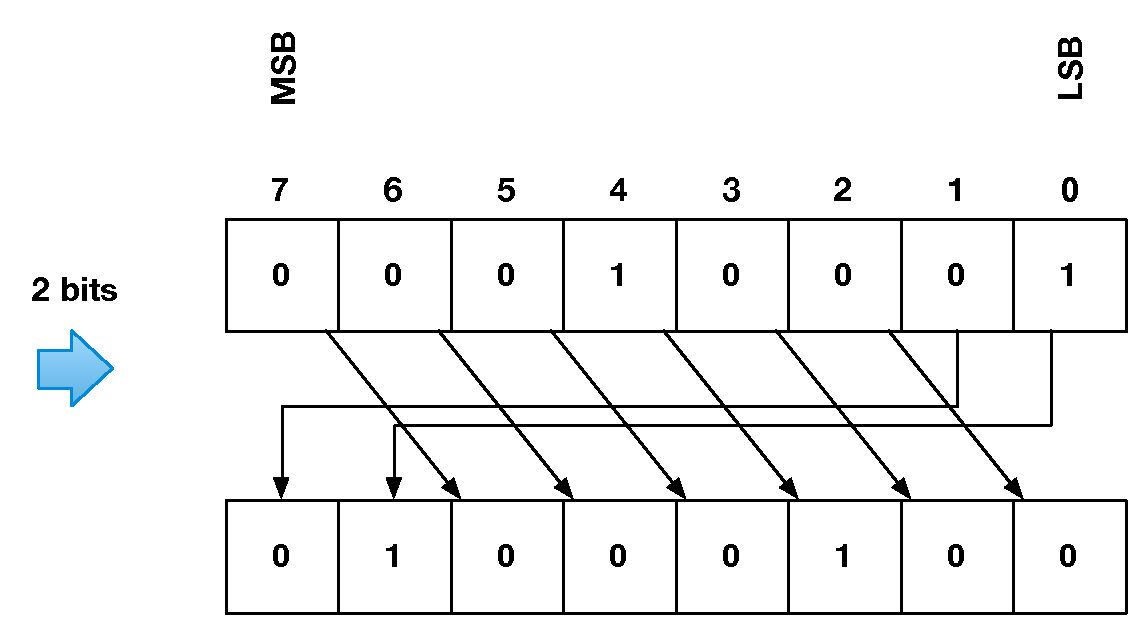
\includegraphics[width=1\textwidth]{./diagrams/r_s_2bits.pdf} \\
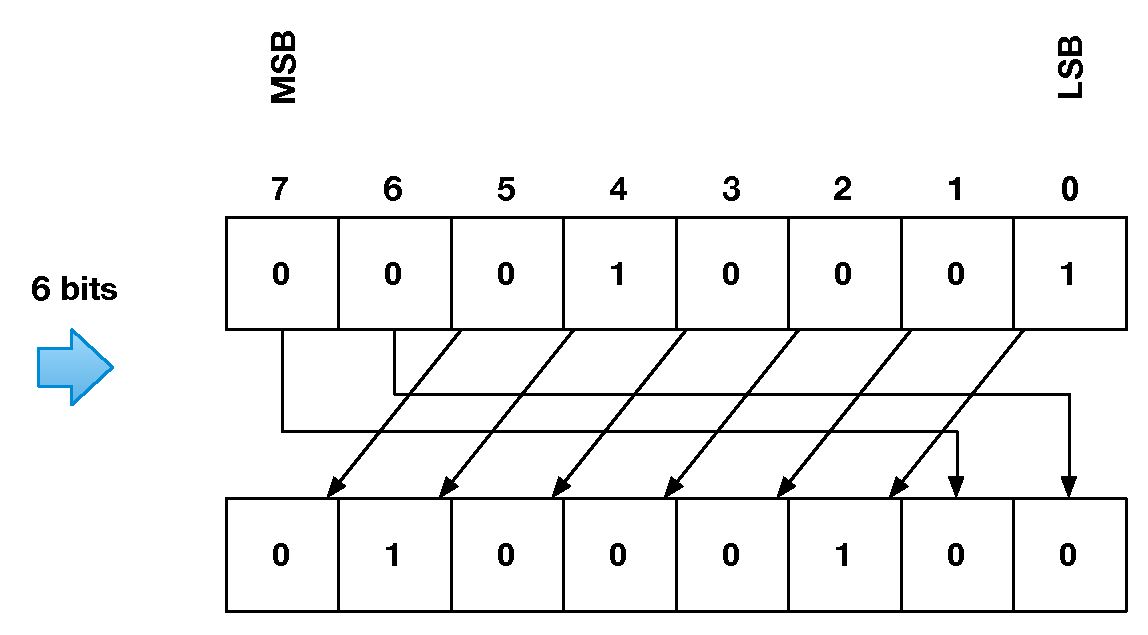
\includegraphics[width=1\textwidth]{./diagrams/r_s_6bits.pdf}
\end{minipage}
}
\subfigure[Different Blocks Shifted Different Bits]{
\begin{minipage}[b]{0.45\textwidth}
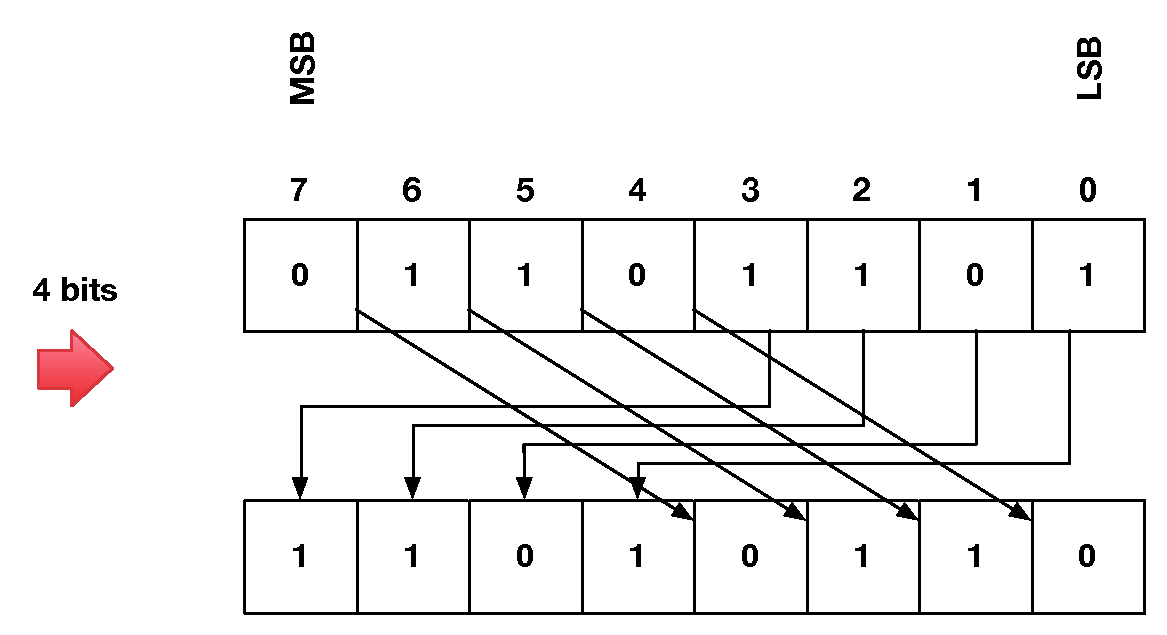
\includegraphics[width=1\textwidth]{./diagrams/r_d_4bits.pdf} \\
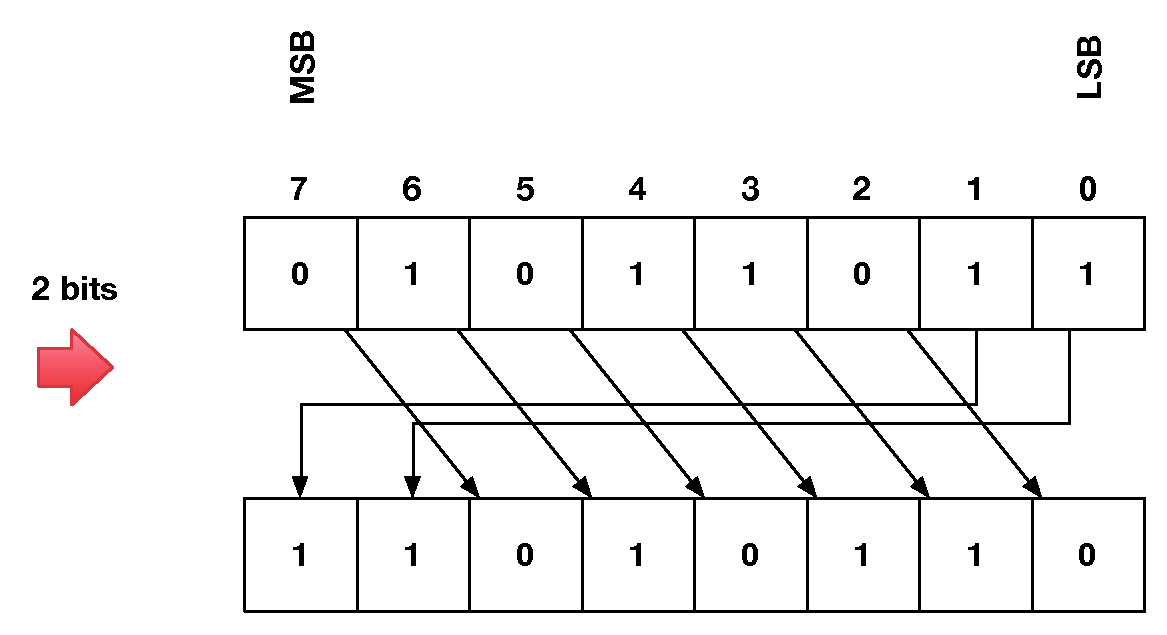
\includegraphics[width=1\textwidth]{./diagrams/r_d_2bits.pdf}
\end{minipage}
}
 \caption{The Examples of Y Block Collision}
 \label{fig: Y-blk-collision}
\end{figure}
Figure $\ref{Y-blk-collision}$ gives the examples of the outputs from shifting
stage that lead tag collision. There are two types of repeated X sets leading to
high probability of tag collision, denoted as sequence-level pattern and
set-level pattern.

\paragraph{The Sequence-level Pattern Collision}
Firstly, we treat blocks as a block sequences, which means in a block sequence, each block has a unique index. The definition of block sequence equality is expressed below:
\begin{defination}
Sequence Equality: Two block sequences X1 and X2 are equal in sequence-level if X$_1$[i] is identical to X$_2$[i] for any i$\in$[1,x].
\end{defination}

Assume the shuffle stage does not work, then the following fact exist:
\begin{itemize}
	\item X1 and X2 are two identical block sequences in sequence-level
\end{itemize}

In block-level rotate shifting stage, a segment from nonce, marked as S, is adopted as the parameter of shifting bits. S is a concatenation of sub-blocks and is denoted as S=(S[1]$\|$S[2]$\ldots$S[x]), where x is the number of blocks in X sequence. The value of S[i] the bits shifted for X[i] block.
For two identical blocks X$_1$[i] and X$_2$[i], the output blocks Y$_1$[i] and Y$_2$[i] are identical if S$_1$[i] is identical to S$_2$[i]. We found that Y$_1$[i] and Y$_2$[i] still have probability to be identical if X$_1$[i] is formed by a repeated short bit segment named pattern. This property is depicted in Proposition 1.1:
%theorem, pattern lead to collision
\begin{theorem}
Let X$_1$[i] and X$_2$[i] be two identical block and len(X$_1$[i])=N, N=2$^n$. Let S$_1$[i] and S$_2$[i] be two distinct shifting bit parameters for X$_1$[i] and X$_2$[i].
Then Y$_1$[i] and Y$_2$[i] can be identical only when X$_1$[i] is formed by repeating a binary bit segment named pattern and marked as P. The length of P len(P) has the following format:
	P\_L = 2$^p$, p$\in$[0,n-1]
\label{sequence-pattern}
\end{theorem}
Base on Theorem $\ref{sequence-pattern}$, we got the following corollaries:
\begin{corollary}
%number of distinct patterns
If a pattern P is not formed by a sub-pattern with shorter length, we call P a distinct pattern with length P\_L. The No. of distinct patterns with length P\_L=2$^p$ is 2$^{2^p}$-2$^{2^{p-1}}$
\label{distinct-pattern}
\end{corollary}
\begin{corollary}
%total number of patterns
Assume the length of a pattern-forming X block is N=2$^n$, then the No. of all possible distinct patterns is 2$^{N/2}$
\label{pattern-no}
\end{corollary}

When the adversary conducts the replay attack on the data concatenated by pattern-formed blocks, the probability that Y block collision is high when shuffle stage does not work. The proof of Theorem $\ref{sequence-pattern}$, Corollary $\ref{distinct-pattern}$ and $\ref{pattern-no}$ is expressed in the appendix. 

\paragraph{The Probability of Tag Collision Under Sequence Pattern Attack}
For two identical X blocks X\_A[i] and X\_B[i], the probability that Y\_A[i]=Y\_B[i] when R\_A[i] and R\_B[i] are randomly generated is marked as  Pr[Y block collision]. 
Pr[Y block collision] is expressed in Theorem $\ref{sequence-prob}$:
%theorem, prob of collide Y from pattern X
\begin{theorem}
Assume for two identical blocks X$_1$[i] and X$_2$[i] the length is N=2$^n$, and the pattern length P$_l$=2$^p$ where p$\in$[0,n-1]. If the pattern contains no internal sub-pattern, then :
\begin{equation}
$$Pr[Y$_1$[i]=Y$_2$[i]] = 1/2$^p$$$
\end{equation}
%If the pattern length in X[i] is identical for any i$\in$[1,x] where x is the number of blocks in X sequence, then:
%\begin{equation}
%$$Pr[Y$_1$[i]=Y$_2$[i]] = (1/2$^p$)$^x$$$
%\end{equation}
\label{sequence-prob}
\end{theorem}

\paragraph{The Set-level Pattern Collision}
%X blocks are from same base
Secondly we treat blocks as a set allowing the existence of identical elements. We give the definition of block set equality below:
\begin{defination}
Set Equality: Two block sets X1 and X2 are identical in set-level if the following properties are met:
\begin{itemize}
	\item X1 and X2 have same number of elements
	\item The number of elements for each distinct value in X1 is identical to the number in X2
\end{itemize}
\end{defination}

When none of block in a X block sequence is formed by repeated pattern, it is impossible to make two Y sequences with block sequence equality by using two distinct s sequences. This assertion can be proved based on the proof of Proposition 1.1. However, we found that it is possible to form two Y sets with block set equality by using two distinct s sequences. The set-level identical Y sets can lead to tag collision directly. This attack is expressed in Theorem $\ref{set-pattern}$:
%theorem, if x blocks are from same base, Y blocks can collide
\begin{theorem}
Let X$_1$[i] and X$_2$[j] be two distinct block and len(X$_1$[i])=len(X$_2$[j])=N, N=2$^n$. Let S$_1$[i] and S$_2$[j] be two distinct blocks of shifting bit parameters for X$_1$[i] and X$_2$[j].
Then Y$_1$[i] and Y$_2$[j] can be identical if and only if X$_1$[i] can be formed by rotate shifting X$_2$[j].
\label{set-pattern}
\end{theorem}
Based on Theorem $\ref{set-pattern}$, we got the following corollary:
\begin{corollary}
For the rotate shifting stage, when the distinct input blocks X$_1$[i] and X$_2$[j] have the property that X$_1$[i] can be formed by rotate shifting X$_2$[j],and the shifting bits parameter S$_1$[i] and S$_2$[j] are distinct, the probability that the output blocks Y$_1$[i] and Y$_2$[j] are identical is:
\begin{equation}
$$Pr[Y$_1$[i]=Y$_2$[j]]= 1/n$$
\end{equation}
\label{set-pattern-cor}
\end{corollary}
 When the adversary conducts replay attack on the memory frame whose data part
is concatenated by blocks that are formated by shifting a common base block,
each element in X1 sequence can be formed by rotate shifting another
element and the probability of forming identical Y sets is high, which will lead
to tag collision. This fact is obvious if the shuffle stage cannot change the
content of input data M.

\paragraph{The Probability of Tag Collision Under Set Pattern Attack}
Assume X1 and X2 are identical in sequence level and each block in X1 can be formed by rotate shifting another block in X1.
From Corollary $\ref{set-pattern-cor}$ we know that for a N-bit block, the size
of domain is 2$^N$ and half of the domain is formed by repeated pattern. This
fact also indicates that half of the domain of a block is not formed with a
pattern, totally 2$^{N/2}$ distinct values. 
%\begin{defination}
%Pr[ SBB only D(X)] =
%\begin{equation}
%2^{n/2} * N^{M-1} / (2^N)^M
%\end{equation}
%\end{defination} 

%Using SBB only X\_A and X\_B, the probability of CIE of Y\_A and Y\_B is marked as Pr[CIE Y Sets] and expressed as the following way:
Assume the X sets under replay attack, marked as X1 and X2, are identical in
sequence level and none of the blocks is formed by a repeated pattern.  If all
the X blocks are formed by rotate shifting a base block which is not consist of
a pattern, we denoted such X1 and X2 sets same base sets, short for SBS sets.

When X1 and X2 are SBS sets, the probability that Y1 and Y2 are identical in set
level if shifting control paramter sets S1 and S2 are randomly generated is
denoted as Pr[Y1 and Y2 are set-level equal $\mid$ X1 and X2 are SBS sets] 
i, short for Pr[Y Sets Collision] 
%\begin{defination}
%Pr[CIE Y Sets] = $$\prod_{i=1,j=1}^M Pr[Y\_A[i] = Y\_B[j]]$$ where M is the No. of elements in a set, i,j$\in$[1,M] and i$\neq$j
%\end{defination} 

%For two randomly generated R\_A and R\_B, the probability that Y\_A and Y\_B are CIE when X\_A and X\_B are SBB only is expressed in the following theorem:
The lower bound of Pr[Y1 and Y2 are set-level equal $\mid$ X1 and X2 are SBS
sets] is expressed in Theorem $\ref{set-prob}$.
%theorem, prob of set-level equal Y if X are same base blocks
\begin{theorem}
\begin{equation}
	  $$Pr[Y Sets Collision]$\geq$($\sum_{K=1}^{min(N,x)}$ (P$_n^k$ * 1/2 * S(x,k)$^2$))/(N$^{2x}$)$$  
\end{equation}
S(x,k) is the Stirling Number with x and k as inputs.

%Pr[CIE Y Sets]:
%\begin{displaymath}
%(\sum_{K=1}^{min(N,M)} \binom{N}{K} * (M!/v1!v2!v3! \cdots vk!) ^ 2 )/(N^M)^2
%\end{displaymath}
\label{set-prob}
\end{theorem}

\paragraph{The Vulnerable Inputs Set of CETD-MAC Under Replay Attack}
%intersection of shuffle and shifting sets lead to highest collision probability
As summarized before, the shuffle stage is vulnerable to inputs that contains
long all-0 or all-1 bit segments. After splitting a input to blocks, shuffle stage cannot effectively change the bit distribution of input blocks and the output of shuffle stage, X blocks, have big probability to be identical to the input.
On the other hand, shifting stage if vulnurable to the input formed with a type of patterns. The patterns can exist in sequence level or set level. The pattern in the input of shifting stage have good chance to induce identical Y sets and directly produce tag collisions. 
We can see that if the input chosen by the adversary for replay attacks is the
in the intersection of vulunrable inputs of shuffle and shifting stage, none of
the stages can effectively randomnize the input data M under replay attack, then there is good chance to form identical Y sets even if the nonce is generated from secure block cipher encryption. 

%\paragraph{The Case of Input Trigging Two Pattern Attacks}
%If the blocks in X set is formed by rotate shifting a base block and this base block is formed by a pattern, then such X set pair X\_A and X\_B can result either IIE or CIE Y set pairs.
%
%Assume the R\_A and R\_B are randomly generated, the probability that Y\_A and Y\_B are SLE is expressed in the following theorem:
%\begin{theorem}
%Assume X\_A and X\_B are both SBB and IPL, R\_A and R\_B are randomly generated,then:
%
%Pr[SLE Y Sets]=
%\begin{displaymath}
%(\sum_{K=1}^{min(N,M)} \binom{N}{K} * (M!/v1!v2!v3! \cdots vk!) ^ 2 )/(N^M)^2
%\end{displaymath}
%\end{theorem}

%\paragraph{The Behaviour of X Blocks from Shuffling Stage}
%\begin{figure}
%\centering
%\subfigure[Only Single Block Equality]{
% \label{fig:y_single_e} %% label for first subfigure
%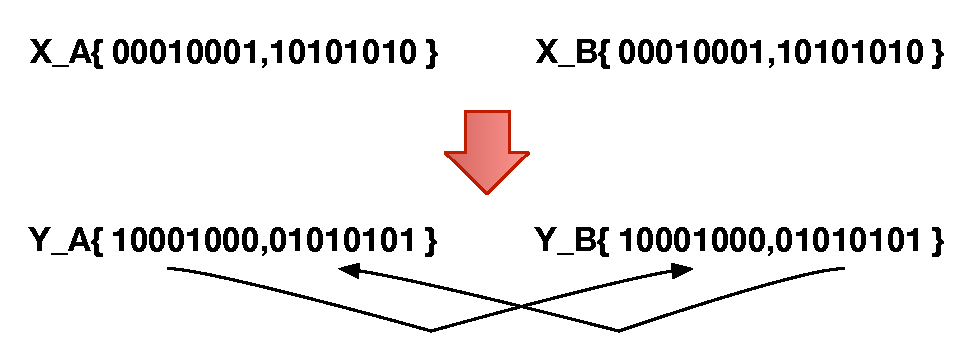
\includegraphics[width=.5\textwidth]{./diagrams/y_single_equality.pdf}
%}
%%\hspace{1in}
%\subfigure[Only Set Level Equality]{
%\label{fig:y_set_e} %% label for second subfigure
%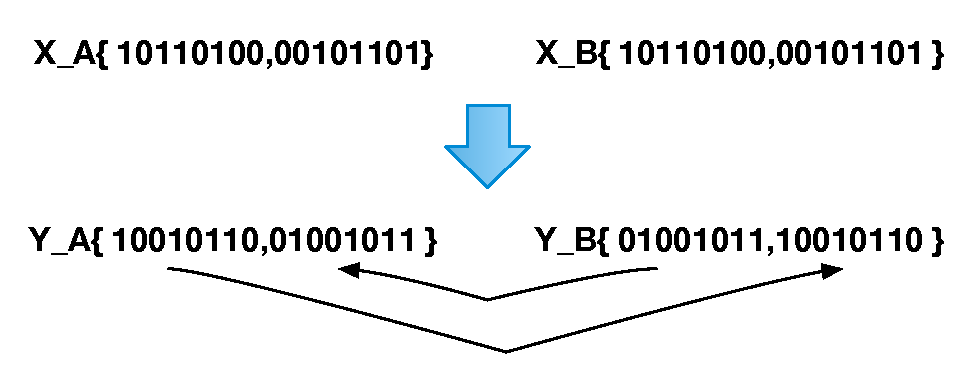
\includegraphics[width=.5\textwidth]{./diagrams/y_set_equality.pdf}
%}
%\caption{X Set Pairs with Only One Type of Y Equality}
% \label{fig:y_e_single} %% label for entire figure
%\end{figure}
%
%\begin{figure}
%\centering
%\subfigure[Single Block Equality Case]{
% \label{fig:y_both_single} %% label for first subfigure
%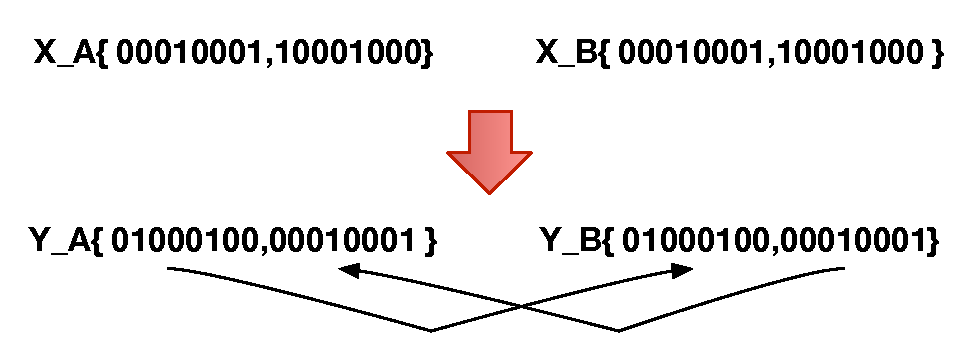
\includegraphics[width=.5\textwidth]{./diagrams/y_both_single.pdf}
%}
%%\hspace{1in}
%\subfigure[Set Level Equality Case]{
%\label{fig:y_both_set} %% label for second subfigure
%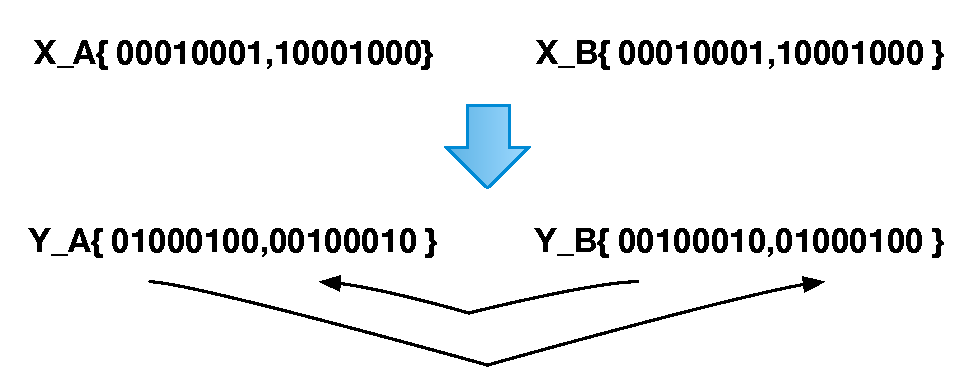
\includegraphics[width=.5\textwidth]{./diagrams/y_both_set.pdf}
%}
%\caption{A X Set Pair with Two Types of Y Equality}
% \label{fig:y_both} %% label for entire figure
%\end{figure}
%In each round of Shuffle stage, two blocks from the output of previous round of shuffle are randomly selected then operate bit segments swapping, which will effect the distribution of bits in the two blocks. After the shuffle stage, the output, X blocks, can be classified to four categories:
%\begin{enumerate}
%	\item Formed by repeated patterns
%	\item Formed by rotate shifting another block in this category
%	\item Contains the properties from categories 1 and 2
%	\item No properties from categories 1 or 2
%\end{enumerate}
%Assume the block cipher used in nonce generation performances like PRF, the number of blocks in each category is effected by the input message M and the rounds of shuffle stage.  

%sequence-pattern
\subsection{Proof of Theorem $\ref{sequence-pattern}$}
This part proves that if two identical block X\_A[i]  and X\_B[i] are shifted different bits and the result blocks remain identical, X\_A[i] is formed by pattern. The pattern length and $\delta$=$\mid$R\_A[i]-R\_B[i] $\mid$ has such correlation:
\begin{itemize}
	\item If $\Delta$ = P\_L then Y\_A[i] = Y\_B[i] where P\_L the length of pattern
\end{itemize}
Assume the length of X\_A[i] is N bits, where N= 2$^n$. When X\_A[i] is formed by a pattern whose length is P\_L = 2$^p$ bits, then the domain of Y\_A[i] has P\_L distinct values. There are N/P\_L distinct R\_A[i] values that shift X\_A[i] to a Y\_A[i].  

%prob of y collide
\subsection{Proof of Theorem $\ref{sequence-prob}$}
For identical each block pair X\_A[i] and X\_B[i], the No. of combination of R\_A[i] and R\_B[i] = N*N, where N is the length a X block. 
If X\_A[i] is formed by pattern, then Y\_A[i]=Y\_B[i] if $\mid$R\_A[i]-R\_B[i]$\mid$ = P\_L * K, where P\_L is the pattern length and K is a positive integer. 
Then for two random R\_A[i] and R\_B[i], Pr[Y\_A[i]=Y\_B[i] $\mid$ X\_A[i] = X\_B[i] \& pattern = P\_L](shoft for Pr[Y\_A[i] = Y\_B[i]]) can be expressed in the following way:
\begin{itemize}
	\item Pr[Y\_A[i]=Y\_B[i]] = N * (N/P\_L)/(N*N) = 1/P\_L
\end{itemize} 

%set-pattern
\subsection{Proof of Theorem $\ref{set-pattern}$}
If two distinct X blocks result two identical Y block. Assume the shift bits parameter blocks are R\_A[i] and R\_B[i]. Then X\_A[i] can be formed by rotate shifting Y\_A[i] for (N-R\_A[i]) mod N bits. X\_B[i] can be formed for (N-R\_B[i]) mod N bits.
X\_B[i] can be formed by rotate shifting X\_A[i] for (R\_A[i] + N-R\_B[i]) mod N bits. Theorem 1.2 proved.

%when x set is sbs, y set is set-level equal
\subsection{Proof of Theorem $\ref{set-prob}$}
As the input sets of rotate shifting stage, X1 and X2, contain the following properties:
\begin{itemize}
	\item X1 and X2 are identical in sequence level
	\item Each block in X1 can be formed by rotate shifint another block in X1 for several bits
\end{itemize}
After the shifting stage, the number of distinct block value in Y1 set, denoted as k, fall in the domain [1,min[N,x]]. For each k, Y1 and Y2 set are identical in set level if the following properties are met:
\begin{itemize}
	\item Y2 blocks have k distinct values 
	\item Assume the k distinct values in Y1 is formed as: value1 has v1 blocks, value2 has v2 blocks, $\ldots$, valuek has vk block and $\sum_{i=1}^k$ vi =x. Then the distribution of k values amount x blocks in Y2 set is same as the distribution in Y1 sets. 
\end{itemize}
For example, assume there is 2 distinct values among 4 blocks in Y1 set, then there are two types of distribution of blocks can be (1,3) or (2,2). For type (1,3) there is four different ways to distribute 4 blocks and for type (2,2) there is three ways.  The number of ways to distribute 2 values to 4 blocks is 4+3=7. If the distribution in Y1 is (1,3), then Y2 set is identical to Y1 set if the distribution of blocks in Y2 is (1,3). 
When there are k distinct values among x blocks, the number of ways to distribute k values to x blocks is know as Stirling Number of Second Type, marked as S(x,k). Assume there are k\_x types of distribution and the number of ways to distribute k values for each distribution type is denoted as V$_1$,V$_2$,$\ldots$,V$_{k\_x}$. Then $\sum_{i=1}^{k\_x}$ V$_i$ = S(x,k)    

For each type of Y1 blocks distribution whose distribution ways number is V$_i$, the number of Y2 sets that are identical to Y1 is V$_i$. Then for each type of distribution, the probability that Y1 and Y2 set are identical in set level can be expressed as:
\begin{equation}
	$$V$_i^2$/(N$^x$)$^2$$$
\end{equation}
Then the probability that if there are k distinct values in Y1 set Y1 and Y2 are identical in set level can be expressed as:
\begin{equation}
	$$P$_N^k$*$\sum_{i=1}^{k\_x}$V$_i^2$/(N$^x$)$^2$$$
\label{k-set-equ-prob}
\end{equation}
As S(x,k) = $\sum_{i=1}^{k\_x}$V$_i$, $\sum_{i=1}^{k\_x}$V$_i^2$ is no less than 1/2 *  S(x,k)$^2$. Then the following inequation stands:
\begin{equation}
	$$P$_N^k$*$\sum_{i=1}^{k\_x}$V$_i^2$/(N$^x$)$^2$ $\geq$ P$_N^k$* 1/2*S(x,k)$^2$/(N$^x$)$^2$$$
\end{equation}
As the domain of k is [1,min(x,N)], then: 
\begin{equation}
$$Pr[Y1 = Y2 $\mid$ S1 and S2 are random] = ($\sum_{k=1}^{min(x,N)}$ (P$_N^k$* 1/2* S(x,k)$^2$))/(N$^x$)$^2$$$
\end{equation}
Theorem $\ref{set-prob}$ is proved.

%\begin{equation}
%	 Pr[Same base X sets leads to set-level equal Y sets] $$$\geq$($\sum_{K=1}^{min(N,x)}$ (P$_n^k$ * 1/2 * S(x,k)$^2$))/(N$^{2x}$)$$  
%\end{equation}
%S(x,k) is the Stirling Number with x and k as inputs.


%\subsection{Proof of Theorem 1.4}
%From Theorem 1.1 we can see that if a X block is formed by a pattern, then the No. of distinct values in the range of Y block is P\_L. While the domain of a R block has N distinct values, then for a block X, there are N/P\_L distinct R values that lead to a Y value.
%
%If a X block is not formed by a pattern, then for each distinct R value, there is a distinct Y value. That means for a given X set that none of the blocks is formed by a pattern, each R set will lead to a distinct Y set. The map between R set and Y set is bijection.
%
%When each R block is randomly generated, the possible combination of R sets is N$^M$. That means for a given X set, the No. of possible Y set is N$^M$.
%
%Assume X\_A and X\_B are IIE and each block can be formed by rotate shifting another block in the set. On the other hand, none of blocks is formed by a pattern. Then the sub-group of blocks in X\_A and X\_B can form CIE with specific R\_A and R\_B set. 
%
%Assume set Y\_A and Y\_B are SLE, then Y\_B is a permutation of Y\_A. This concept can be modeled in the following way:
%\begin{itemize}
%	\item Assume the M elements in Y\_A contain K distinct values. The No. of the elements that have each value are marked as v1,v2...vk.
%	\item IF the elements in Y\_B are a permutation of the elements in Y\_A, then Y\_A and Y\_B are SLE.
%\end{itemize}
%
%Based on the basic concept in Combinatorics, the No. of a permutation of Y\_A that contains K distinct value can be expressed in the following equation:
%\begin{defination}
%No. of Permutation with K distinct Values:
%\begin{displaymath}
%\binom{M}{v1} * \binom{M-v1}{v2} * \binom{M-v1-v2}{v3} \cdots * \binom{vk}{vk} = M!/v1!v2!v3! \cdots vk!
%\end{displaymath}
%\end{defination}
%As any one of the elements in X set can be formed by rotate shifting another element, then the No. of distinct values of M elements, K, various from 1 to M. If Y\_A has K distinct values, the No. of possible combination of these K elements in Y\_A can be expressed as Com\_Y\_A:
%\begin{defination}
%Com\_Y\_A:
%\begin{displaymath}
%M!/v1!v2!v3! \cdots vk!
%\end{displaymath} 
%\end{defination} 
%
%For each case of Y\_A in Com\_Y\_A, the No. of Y\_B to form SLE is also Com\_Y\_A. Then if Y\_A has K distinct values, Pr[CIE Y sets] can be expressed as:
%\begin{defination}
%Pr[CIE Y Sets]:
%\begin{displaymath}
% \binom{N}{K} * (M!/v1!v2!v3! \cdots vk!) ^ 2 /(N^M)^2
%\end{displaymath}
%\end{defination}
%If R\_A and R\_B are randomly generated, then the value of K various from 1 to M. We do th sum to get the expression in Theorem 1.4
%\begin{defination}
%Pr[CIE Y Sets]:
%\begin{displaymath}
%(\sum_{K=1}^{min(N,M)} \binom{N}{K} * (M!/v1!v2!v3! \cdots vk!) ^ 2 )/(N^M)^2
%\end{displaymath}
%\end{defination}

%\subsection{Proof of Theorem 1.5}
%If the element contains both the properties of CIE and IIE, then the following properties:
%\begin{itemize}
%	\item For two distinct sets R\_A and R\_B, Y\_A and Y\_B can be IIE
%	\item For each value of a Y block, there are N/P\_L distinct R block that can shift X to this Y. That means for a distinct Y set, the No. of R sets is not one.
%	\item For two distinct sets R\_A and R\_B, Y\_A and Y\_B can be CIE
%\end{itemize}
%Base on the Theorem 1.1, if the X block is formed by pattern, then the No. of values in the range of Y is P\_L, base on theorem 1.4, the Pr[SLE Y sets] can be expressed as:
%\begin{defination}
%Pr[SLE Y Sets:]:
%\begin{displaymath}
%\binom{P\_L}{K} * (M!/v1!v2!v3! \cdots vk!) ^ 2 )/(P\_L^M)^2
%\end{displaymath}
%\end{defination}
%
%If R\_A and R\_B are randomly generated, then the value of K various from 1 to M. We do th sum to get the expression in Theorem 1.5
%\begin{defination}
%Pr[SLE Y Sets]:
%\begin{displaymath}
%(\sum_{K=1}^{min(P\_L,M)} \binom{P\_L}{K} * (M!/v1!v2!v3! \cdots vk!) ^ 2 )/(P\_L^M)^2
%\end{displaymath}
%\end{defination}
%\subsection{Proof of Theorem $\ref{set-prob}$}


%\subsection{Security Enhanced CETD-MAC}
%In this section we provide an modification of original CETD-MAC. Our approach does not require additional component or information to the original CETD-MAC. We then prove that the optimized CETD-MAC can fix the weakness and protect input message from replay attack.
%\paragraph{Inspiration}
%As depicted above, if a input message is consisted of blocks formed with a type of pattern and the proportion of 0s and 1s in the message is extremely unbalanced, the message cannot be effectively randomized by neither the shuffle stage nor the shifting stage. That means the message has high probability to induce identical Y sets or Y sequences under replay attack. The identical Y sets or Y sequences will directly induce tag collision then succeed the replay attack. 
%\paragraph{Solution}
%As discussed above, the reason of high probability of tag collision for some specific inputs
%under replay attack is that neither the shuffle or the shift stage can
%randomnize the input then the Y sets collide easily. The solution should be
%randomnize the outputs from shuffle, shift or the xor stage.
%
%As the the outputs from shuffle and shift stage is consist of multiple blocks,
%all the blocks should be randomnized, otherwise the patterns existing in the
%input data M remains in some blocks.  
%The cost and lattency of such a optimization of CETD-MAC is dependent on the
%length of input data M, which is not efficient if the input is long.
%
%Our solution is expressed as below:
%\begin{itemize}
%	\item Xor a random block to the output of XOR operation
%	\item Assume the MSB bits of nonce are adopted as control paramters for
%shuffle and shifting stage, we choose LSB bits on the nonce as the random block 
%	\item The random block is denoted as Mask\_Tag, and len(Mask\_Tag) =
%len(Tag).
%\end{itemize}
%We denote the output of original CETD-MAC scheme in our optimized scheme T\_xor
%and tag of optimized scheme for T, the probability of tag collision of optimized scheme is
%expressed as Pr[tag collision].  
%
%The computation of Pr[tag collision] is expressed below:
%\begin{equation}
%	$$Pr[tag collision] = Pr[Mask\_Tag1 $\oplus$ T\_xor1 $\oplus$ Mask\_Tag2
%$\oplus$  T\_xor2 =0] $$
%	$$=Pr[Mask\_Tag1 $\oplus$ Mask\_Tag2 = k $\mid$ k = T\_xor1 $\oplus$ T\_xor2
%]$$
%\end{equation}
%As nonce is the output of block cipher encryption, the big segment of nonce is
%assumed as a output from PRF. Then Pr[tag collision] = 1/$2^{len(T)}$. This
%result means our optimized scheme can assure the randomness of tags under replay
%attack and is secure. 


\end{document}
